\setchapterpreamble[u]{\margintoc}
\chapter{Cenni alla teoria dei numeri}
\labch{chapter3}

\begin{definition}
Sia \(m \ge 1\) un intero. Gli interi \(a\) e \(b\) sono \textit{congruenti modulo m} se la loro differenza \(a-b\) è divisibile per \(m\). La formula 
\[a \equiv b \pmod m\]
indica che \(a\) e \(b\) sono congruenti in modulo \(m\).
\end{definition}

\noindent\\ Un esempio può essere l'aritmetica delle "ore". Usando il modulo $m = 12$:
\begin{align*}
    6+9=15 \equiv 3 \pmod{12} \hspace{2cm} 2-3=-1 \equiv 11 \pmod{12}
\end{align*}

\noindent I numeri che soddisfano 
\begin{align*}
    a \equiv 0 \pmod m
\end{align*}
\noindent sono tutti i numeri divisibili per $m$, ovvero tutti i suoi multipli $km$.\\

\noindent Dati $m \ge 1$ e $a, b$ interi, allora
\begin{align*}
    a \cdot b = 1 \pmod m
\end{align*}

\noindent se e solo se $GDC(a, m) = 1$.\\

\noindent Dato $GDC(a, m) = 1$ allora esiste un inverso $a^{-1}$ di $a \pmod m$ tale per cui $a^{-1}a \equiv 1 \pmod m$. \\

\noindent \underline{Esempio}: dati $m = 5$ e $a = 2$, $GDC(5, 2) = 1$ e quindi esiste un inverso di $2 \pmod 5$. L'inverso è $3$, in quanto $2\cdot 3 \equiv 1 \pmod 5$.
\\

\noindent Se $a$ diviso $m$ ha quoziente $k$ e resto $r$, allora questo può essere riscritto come:
\begin{align*}
    a = m \cdot k + r \hspace{1cm} \text{con } 0 \le r < m
\end{align*}

\section{Algebra modulo n}
L'insieme $Z_n$ viene definito come l'insieme delle classi di equivalenza $[0]$, $[1]$, $...$, $[n-1]$ di una relazione che dice che ${a}$ è congruente a ${b}$ se e solo se ${a}$ modulo $n$ è uguale a ${b}$ modulo ${n}$, dove il modulo è il resto della divisione per ${n}$:

\begin{align*}
    Z_n = \{[0], [1], [2], ..., [n-1]\}\\
    a \equiv_n b \Longleftrightarrow a \pmod n= b \pmod n
\end{align*}

\noindent Quando ho una relazione di equivalenza posso costruire gli insiemi degli insiemi che sono equivalenti tra di loro. L'insieme degli insiemi che sono equivalenti tra di loro forma una partizione dell'insieme di partenza; gli elementi della partizione vengono chiamati classi di equivalenza e si denotano mettendo tra parentesi quadre \textit{[ ]} un elemento della classe di equivalenza. 

Quindi quando parlo di un'algebra modulo n parlo di un insieme $Z_n$ che è l'insieme delle classi di equivalenza della divisione per n; ogni singola classe di equivalenza può essere rappresentata da un qualsiasi elemento che vi appartiene. Posso infatti anche scrivere:
\begin{align*}
    Z_n = \{0, 1, 2, ..., n-1\}
\end{align*}

\noindent ovvero i primi \textit{n} numeri naturali a partire dallo $0$. La rappresentazione canonica in un'algebra a modulo n è un numero compreso tra $0$ e $n-1$.\\

\noindent\fbox{%
    \parbox{\textwidth}{%
    Il cifrario di Cesare lavora shiftando ogni lettera dell'alfabeto di un numero fissato di posizioni. Lo shift può essere descritto con un'aritmetica modulo $26$:
    \begin{align*}
        (Cyphertext) \equiv (Plaintext\_Letter) + (Secret\_Key) \pmod{26}\\
        (Plaintext\_Letter) \equiv (Cyphertext) - (Secret\_Key) \pmod{26}
    \end{align*}
    }
}

\paragraph*{Numeri razionali} Questo tipo di notazione è già stata usata per definire i numeri razionali, che sono classi di equivalenza su coppie di numeri naturali dove due coppie sono equivalenti se hanno gli stessi prodotti incrociati (prodotto dei medi uguale prodotto degli estremi). 

Ad esempio la coppia ${\frac{a}{b}}$ è un rappresentate delle coppie ${\frac{2a}{2b}}$, ${\frac{3a}{3b}}$ e così via. Tra tutti i possibili rappresentati di una classe ce n'è uno canonico, dove in questo caso è l'oggetto che si ottiene dalla riduzione ai minimi termini.

\subsection{Somma nell'insieme $Z_n$} Definisco ora l'operazione di somma $(Z_n, +)$:
\begin{align*}
    [a] + [b] = [a + b]
\end{align*}

\noindent Questa definizione dice che la somma delle classi di equivalenza di $[a]$ e $[b]$ è uguale alla classe di equivalenza della somma di $a$ e $b$ $[a+b]$. Si considera buona solo se il risultato è indipendente dagli elementi che prendo come rappresentanti delle due classi da sommare. Questa operazione di somma gode di una serie di proprietà:
\begin{itemize}
    \item La somma è commutativa: $\forall a, b: a+b=b+a$;
    \item La somma è associativa: $\forall a, b, c: (a+b)+c=a+(b+c)$;
    \item La somma ammette un elemento neutro $e$: $\exists \ e \forall a: a+e=e+a=a$ con $e= 0 \lor n$. Nell'algebra modulo n vale anche $n$ (e anche $2n$, $3n$, ...) come elemento neutro in quanto è un elemento appartenente alla classe di equivalenza di $0$. Similmente, nei razionali l'elemento neutro è si $1$, ma anche ${\frac{2}{2}}$, ${\frac{3}{3}}$ e così via;
    \item La somma ammette l'elemento inverso: $\forall a \ \exists a^{-1} : a+a^{-1} = a^{-1}+a = e$. L'inverso di un numero è quel numero che messo nell'operazione di interesse con il numero originale mi dà l'elemento neutro. Ad esempio, il numero inverso nella somma è il negativo di quel numero (che nei naturali non esisterebbe, ed è per quello che si estende con gli interi); nei razionali l'inverso di $\frac{a}{b}$ nella moltiplicazione è $\frac{b}{a}$ (negli interi l'inverso della moltiplicazione non c'è, e quindi si estende con i razionali). 
    
    In questo caso, posso scrivere l'elemento in più modi: $a^{-1}=-a=n-a$.
\end{itemize}

\noindent Una "cosa" che ha le proprietà di associatività, elemento neutro e elemento inverso è detta \textbf{gruppo}, mentre una che gode di tutte e quattro le proprietà è detta \textbf{gruppo abeliano}. Quindi l'insieme $Z_n$ con l'operazione di somma è un gruppo.

Gli interi con l'operazione di moltiplicazione non formano un gruppo, in quanto non esiste l'elemento inverso. I razionali sono un gruppo con la somma, ma non con il prodotto, in quanto non esiste l'inverso dello $0$. Se ai razionali però rimuovo l'elemento neutro della somma, diventano un gruppo anche con il prodotto.

I razionali sono un campo. Un insieme è un \textbf{campo} se è un gruppo con la somma e col prodotto a cui è rimosso l'elemento neutro della somma.

\subsection{Prodotto in ($Z_n \backslash \{0\}, *$)} La moltiplicazione è definita coma segue:
\begin{align*}
    [a] * [b] = [a*b]
\end{align*}

\noindent Il prodotto, in $Z_n$ senza lo $0$, è commutativo e ha l'elemento neutro, ma non ha (sempre) l'elemento inverso:
\begin{align*}
    &Z_{15} \backslash \{0\} = \{1, 2, 3, ..., 14\}\\
    &\text{L'inverso moltiplicativo di $2$ è $8$: }2*8 = 16 \equiv 1 \pmod{15}\\
    &\text{L'inverso moltiplicativo di $3$ non esiste}
\end{align*}

\noindent In generale lavorando con l'operazione di moltiplicazione nei gruppo in modulo n si perde l'elemento inverso. Una possibilità è prendere un sottoinsieme di $Z_n$ che garantisce l'elemento inverso.

\section{Insieme $Z^*_n$}
Sottoinsieme di $Z_n$ tale per cui:
\begin{align*}
    Z^*_n = \{a \in (Z_n \backslash \{0\}) \mid MCD(a, n) = 1 \}
\end{align*}

\noindent dove $MCD$ indica il massimo comun divisore. Questo insieme contiene elementi $a$ di $Z_n$ tali per cui il massimo comun divisore tra $a$ e $n$ è $1$. Contiene gli elementi che sono relativamente primi con $n$. 

Se moltiplico tra loro due elementi di $Z^*_n$ ho la garanzia di ottenere ancora un elemento di $Z^*_n$ (se i due numeri non hanno fattori in comuni con $n$, allora anche il loro prodotto non avrà fattori in comune con $n$). La moltiplicazione quindi qui è \textbf{chiusa}. L'elemento neutro è $1$.

\begin{theorem}
    \(\forall a, b \  \exists x, y : ax + by = MCD(a, b)\).
\end{theorem}

\noindent Se $a \in Z^*_n$, allora:
\begin{align*}
     \exists x, y : \ &ax + ny = 1\\
                    &ax = 1 - ny\\
                    &ax \equiv 1 \pmod n
\end{align*}

\noindent Quindi la classe a cui appartiene $x$ è l'inverso di $a$. Ho confermato che $Z^*_n$ con il prodotto è un gruppo.

\paragraph{Funzione di Eulero $\varphi$} Dato l'insieme $Z_n^*$ allora:
\begin{align*}
    \varphi(n) &= \ \mid Z_n^* \mid \\\\
    \varphi(p) &= \ \mid p-1 \mid \\
    \varphi(pq) &= \ \mid (p-1) \cdot (q-1) \mid
\end{align*}

\noindent Sia $n = pq$ e $x<n$ un numero a caso. La probabilità che $x \in Z_n^*$ è:
\begin{align*}
    Pr[x \in Z_n^*] = \frac{(p-1)(q-1)}{pq} = \frac{p-1}{p} \cdot \frac{q-1}{q} > \frac{1}{4}
\end{align*}

\section{Generatore di un gruppo}
Sia $(G, *)$ un gruppo finito, e sia $g$ un elemento di $G$, allora se prendo la serie di elementi
\begin{align*}
    g = g^1, g*g=g^2, g*g*g=g^3, ..., g^{|G|}, g^{|G|+1}, ...
\end{align*}
\noindent per il pumping lemma vi è almeno un elemento ripetuto e la sequenza diventa quindi ciclica (dall'elemento ripetuto in poi continua a ripetere la sotto-sequenza).

\begin{theorem}
    \(\forall \text{ Gruppo } G \text{ finito } \forall a \in G : a^{|G|} = 1\).
\end{theorem}

\noindent Per questo teorema, se prendo un elemento qualsiasi di un gruppo e lo elevo alla cardinalità del gruppo, otteno $1$. Quindi in questa catena l'elemento neutro c'è, che sarebbe $g^0 = 1$.

Se prendo tutte le potenze di $g$ ottengo un \textbf{sottogruppo} di $G$, che è un sottoinsieme dell'insieme $G$ che resta un gruppo. Se il sottogruppo che ottengo è l'intero gruppo $G$, allora $G$ è \textbf{ciclico} e $g$ è un \textbf{generatore} di $G$.

\begin{theorem}[Teorema di Lagrange]
    Se $G'$ è un sottogruppo di $G$, allora $|G'| \bigg| |G|$, ovvero il numero di elementi di $G'$ è divisore del numero di elementi di $G$.
\end{theorem}

\noindent \\ \underline{Esempio}\\

\noindent Provo ora a costruire tutti i sottogruppi di $Z^*_{15} = \{1, 2, 4, 7, 8, 11, 13, 14\}$:

\begin{align*}
    &\underline{1}\\
    &\underline{2}*2=4, \underline{4}*2=8, \underline{8}*2=16, 16 \pmod{15} = \underline{1}\\
    &\underline{4}*4=16, 16 \pmod{15} = \underline{1}\\
    &\underline{7}*7=49, 49 \pmod{15} = \underline{4}, 4*7=28, 28 \pmod{15} = \underline{13}, 13*7 = 91 \pmod{15} = \underline{1}\\
    &8, 4, 2, 1\\
    &11, 1\\
    &13, 4, 7, 1\\
    &14, 1
\end{align*}

\noindent Ho confermato che la cardinalità di tutti i generatori divide la cardinalità dell'insieme originale, ma nessuno di questi generatori è ciclico. Esistono generatori ciclici? Si, almeno quando $n$ è primo. In generale dato $p$ numero primo, il rispettivo insieme sarà $Z^*_{p} = \{1, ..., p-1\}$.

\begin{theorem}
    I gruppi \(Z_p^*\), con \(p\) numero primo, sono gruppo ciclici.
\end{theorem}

\noindent \underline{Esempio}\\

\noindent Provo ora a cercare un generatore di $Z^*_{7} = \{1, 2, 3, 4, 5, 6\}$:
\begin{align*}
    &1 \rightarrow 1 \text{ non è un generatore}\\
    &2, 4, 1 \rightarrow 2 \text{ non è un generatore}\\
    &3, 2, 6, 4, 5, 1 \rightarrow 3 \text{ è un generatore}
\end{align*}

\begin{theorem}[Fermat’s Little Theorem]
    Sia \(p\) un numero primo e sia \(a\) un intero (con \(ka\) un possibile multiplo di $a$). Allora
    \begin{align*}
        a^{p-1} \equiv 
        \begin{cases}
                1 \pmod p & \text{ se } p \ne ka\\
                0 \pmod p & \text{ se } p \big| ka
        \end{cases}
    \end{align*}
\end{theorem}

\noindent \underline{Esempio}\\

\noindent Vediamo la liste delle potenze dei numeri $1, 2, ..., 6$ in modulo con il numero primo $7$:

\begin{center}
     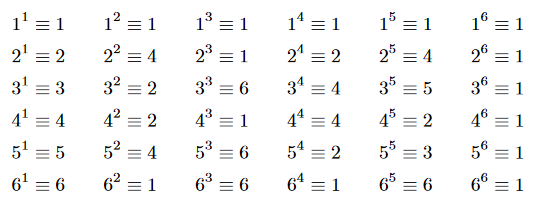
\includegraphics[width=1\textwidth]{images/6.png}
\end{center}

\noindent Si può vedere che la colonna di destra, quella degli $a^{6}$, produce tutti $1$.

\section{Numero quadrato}

\begin{definition}
Sia \(p\) un numero primo dispari e sia $a \in Z^*_p$. Si dice che \(a\) è un residuo quadratico di modulo \(p\) se \(a\) è un quadrato modulo \(p\), ovvero esiste un numero \(c\) tale che \[c^2 \equiv a \pmod p\]
In caso contrario \(a\) è detto non residuo quadratico modulo \(p\).
\end{definition}

\noindent Dato $(G, *)$, un gruppo $G$ con l'operazione $*$, il numero di quadrati che contiene è esattamente uguale a $\frac{p-1}{2}$, ovvero a tutti e soli gli elementi $g^{2i}$ (elementi con esponente pari). Ogni elemento $g^{2i}$ ha due radici:
\begin{align*}
 	g^{2i}=
 	    \begin{cases}
 	   g^i \\ 
 	    g^{i+\frac{p-1}{2}} \hspace{1cm} \rightarrow (g^{i+\frac{p-1}{2}})^2 = g^{2i}\cdot g^{p-1} = g^{2i}\cdot 1
        \end{cases} 
\end{align*}

\noindent Poiché le due radici di un numero sono opposte, allora $g^{\frac{p-1}{2}} \equiv -1$. Quindi elevare un generatore alla cardinalità del gruppo dà l'unità, mentre elevarlo alla metà della cardinalità dà l'opposto dell'unità.

\paragraph{Quadrati in $Z_{pq}^*$} Dato $Z_{pq}^*$, con $p, q$ numeri primi, il numero di quadrati contenuto nell'insieme è $\frac{\varphi}{4}$, ovvero il numero di quadrati comuni a $Z_{p}^*$ e $Z_{q}^*$.

\noindent Dato $p$ numero primo, come è possibile capire se un dato numero $a$ sia uguale a un quadrato modulo $p$? Escludendo il risolvere il problema del logaritmo discreto per $a$ e verificare se il risultato è pari o dispari, un modo per farlo è verificare se $x_i^2 = a$, per ogni $x_i \in 0, 1, 2, 3, 4, ..., p-1$. Esistono modi più efficienti? 

\begin{definition}[Simbolo di Legendre]
Il simbolo di Legendre è definito come segue:
\begin{align*}
    \left( \frac{a}{p} \right) &= a^{\frac{p-1}{2}} \pmod p\\\\
    \left( \frac{a}{p} \right) &= 
    \begin{cases}
        1 & \text{ se } a \text{ è un residuo quadratico modulo } p\\
        -1 & \text{ se } a \text{ è un non residuo quadratico modulo } p\\
    \end{cases}
\end{align*}
\end{definition}

\noindent Infatti:
\begin{itemize}
    \item Sia $a = g^{2i}$, ovvero un quadrato, allora
\begin{align*}
    a^{\frac{p-1}{2}}= (g^{2i})^{\frac{p-1}{2}} = (g^i)^{(p-1)} = 1
\end{align*}
\item Sia $a = g^{2i+1}$, ovvero un non quadrato, allora
\begin{align*}
    a^{\frac{p-1}{2}}= (g^{2i+1})^{\frac{p-1}{2}} = (g^{2i})^{\frac{p-1}{2}} \cdot g^{\frac{p-1}{2}} = 1 \cdot (-1) = -1
\end{align*}
\end{itemize}

\noindent Il simbolo di Legendre ritorna $1$ se $a$ è un quadrato modulo $p$ o $-1$ se non lo è. 

Si può calcolare questo algoritmo in tempo polinomiale, con numeri da migliaia di bit? Il simbolo di Legendre consiste nel calcolare una potenza, che equivale nella pratica a calcolare una serie di moltiplicazioni. Quindi la domanda diventa: esiste un algoritmo per eseguire moltiplicazioni in tempo polinomiale? Si, il \textbf{Fast Power Algorithm}. 

Praticamente il simbolo di Legendre permette di ottenere il bit meno significativo del numero, che permette di capire immediatamente se il numero è pari (0) o dispari (1).\\

\noindent Dato $n=pq$, come è possibile capire se un numero $a$ è un quadrato in $Z_n^*$? Il modo più semplice sarebbe fattorizzare $n$ in $p$ e $q$ e calcolare il simbolo si Legendre di $a$ rispetto ai due fattori. Poichè fattorizzare è difficile (non esistono algoritmi efficienti), allora anche determinare se $a \in Z_n^*$ dovrebbe essere difficile. In realtà non è proprio così. 

Il simbolo di Jacobi, una generalizzazione del simbolo di Legendre, permette di determinare $\left(\frac{a}{n} \right)$ senza dover fattorizzare.
\begin{definition}[Simbolo di Jacobi] Siano \(a\) e \(n\) due interi, con \(n\) dispari e positivo. Supponendo che la fattorizzazione di \(n\) in numeri primi sia 
\begin{align*}
    n = p_1^{e_1} \cdot p_2^{e_2} \cdot ... \cdot p_t^{e_t}
\end{align*}

\noindent allora il simbolo di Jacobi \(\left(\frac{a}{n}\right)\) è definito dalla formula 
\begin{align*}
    \left(\frac{a}{n}\right) = \left(\frac{a}{p_1}\right)^{e_1} \left(\frac{a}{p_2}\right)^{e_2} ... \left(\frac{a}{p_t}\right)^{e_t}
\end{align*}
\end{definition}

\noindent Il simbolo di Jacobi $\left(\frac{a}{n}\right)$ gode delle seguenti proprietà:
\begin{align*}
    \left(\frac{a}{n_1n_2}\right) = \left(\frac{a}{n_1}\right)\left(\frac{a}{n_2}\right)
\end{align*}
\begin{align*}
        \left(\frac{a_1a_2}{n}\right) = \left(\frac{a_1}{n}\right)\left(\frac{a_2}{n}\right)
\end{align*}

\noindent Se $n$ è un numero primo, allora il simbolo di Jacobi equivale al simbolo di Legendre. Se scompongo $n$ in numeri primi, allora ogni simbolo di Jacobi $\left(\frac{a}{p_i}\right)$ mi ritorna $1$ o $-1$:
\begin{align*}
    \left(\frac{a}{n}\right) &= \left(\frac{a}{pq}\right) = \left(\frac{a}{p}\right)\left(\frac{a}{q}\right)
\end{align*}

\noindent Il simbolo di Jacobi, come detto all'inizio, è risolvibile con un algoritmo polinomiale che non richiede la scomposizione in fattori primi.

Tornando al caso iniziale $n = pq$, nel calcolo del simbolo di Jacobi $\left(\frac{a}{pq}\right)$ si possono incontrare tre casi:
\begin{enumerate}
    \item $a$ è un quadrato sia in $Z_p^*$ che in $Z_q^*$ (probabilità $\frac{1}{4}$):
        \begin{align*}
            \left(\frac{a}{pq}\right) = \left(\frac{a}{p}\right)\left(\frac{a}{q}\right) = 1 \cdot 1 = 1
        \end{align*}
    \item $a$ è un quadrato sia in $Z_p^*$ ma non $Z_q^*$ (probabilità $\frac{1}{4}$) o viceversa (probabilità $\frac{1}{4}$):
        \begin{align*}
            \left(\frac{a}{pq}\right) = \left(\frac{a}{p}\right)\left(\frac{a}{q}\right) = 1 \cdot (-1) = -1\\\\
            \left(\frac{a}{pq}\right) = \left(\frac{a}{p}\right)\left(\frac{a}{q}\right) = (-1) \cdot 1 = -1
        \end{align*}
    \item $a$ non è un quadrato sia in $Z_p^*$ ne in $Z_q^*$ (probabilità $\frac{1}{4}$):
        \begin{align*}
            \left(\frac{a}{pq}\right) = \left(\frac{a}{p}\right)\left(\frac{a}{q}\right) = (-1) \cdot (-1) = 1
        \end{align*}
\end{enumerate}

\noindent Dai tre casi sopra, si può capire che il simbolo di Jacobi è limitato rispetto al simbolo di Legendre, in quanto è in grado solamente di decidere se un numero è un non quadrato nel caso particolare in cui è un quadrato in $Z_p^*$ e non quadrato in $Z_q^*$ (o viceversa).
Il simbolo di Jacobi si può quindi riassumere così:
\begin{align*}
    \left(\frac{a}{n}\right)=
 	    \begin{cases}
 	   -1& \mbox{ $a$ è un non quadrato}\\ 
 	    1& \mbox{ non so}
        \end{cases} 
\end{align*}

\noindent Di conseguenza, determinare se dato un numero con simbolo di Jacobi $1$ è quadrato o non quadrato è un problema difficile.

\section{Fast Powering Algorithm}
In molti crittosistemi come RSA e DH, i due attori necessiteranno di calcolare potenze di grandi dimensioni. Un modo per calcolare ad esempio $a^b \pmod n$ è per moltiplicazioni ripetute di $a$. Quindi
\begin{align*}
    a_1 \equiv a \pmod n \hspace{1cm} a_2 \equiv a_1 \cdot a \pmod n \hspace{1cm} ... \hspace{1cm} a_{b} \equiv a_{b-1} \cdot a \pmod n
\end{align*}

\noindent Se $b$ è un numero elevato, l'algoritmo non è pratico. Un modo migliore per calcolare la potenza è usare l'espansione binaria di $b$ per convertire il calcolo in una successione di quadrati e moltiplicazioni.\\
 
\noindent Ad esempio, dato $b = 75 = 1001011$, le rispettive potenze saranno:
 \begin{align*}
     2^6+2^3+2^1+2^0 
 \end{align*}
 \noindent Quindi:
 \begin{align*}
     a^b = a^{2^6+2^3+2^1+2^0} = a^{2^6} *a^{2^3}*a^{2^1}*a^{2^0}
 \end{align*}

\noindent Questa sequenza di valori è semplice da calcolare in quanto ogni numero nella sequenza è il quadrato del precedente:
\begin{align*}
    a^{2^0} &= a\\
    a^{2^1} &= a*a\\
    a^{2^2} &= a^{{2^1}^2}
\end{align*}

\noindent Questo metodo è chiamato \textbf{iterative squaring} e permette di calcolare le potenze in un numero di moltiplicazioni proporzionale ai bit di $b$. Calcola via via le potenze di $a$, elevate a potenze di 2, e verifica a vedere se il corrispondente bit dell'espressione binaria di $b$ vale $0$ o $1$: se vale $0$ non fa nulla, se vale $1$ moltiplica il risultato parziale per la potenze che ha calcolato.

\begin{algorithm}[H]
\caption{Iterative squaring EXP(a, b)}\label{alg:cap}
\begin{algorithmic}
\State $y \gets 1$
\State $t \gets a$
\While{$b \neq 0$}
\If{$b \% 2 == 1$}
    \State $y \gets y \times t$
\EndIf
    \State $b \gets b / 2$
    \State $t \gets t \times t$
\EndWhile
\end{algorithmic}
\end{algorithm}

\noindent Complessità dell'algoritmo, in funzione dei bit di $a$ e $b$:

\begin{algorithm}[H]
\caption{Iterative squaring EXP(a, b) - complessità}\label{alg:cap}
\begin{algorithmic}
\State $y \gets 1$ \Comment{lineare nel numero di bit di b}
\State $t \gets a$ \Comment{lineare, devo copiare tutti i bit di a}
\While{$b \neq 0$} \Comment{lineare}
\If{$b \% 2 == 1$} \Comment{costante, guardo il bit meno significativo }
    \State $y \gets y \times t$ \Comment{quadratico nella lunghezza del numero}
\EndIf
    \State $b \gets b / 2$ \Comment{lineare o costante in base a come salvo il numero}
    \State $t \gets t \times t$ \Comment{quadratico}
\EndWhile
\end{algorithmic}
\end{algorithm}

\noindent L'algoritmo è quindi di complessità cubica, con il corpo del while è quadratico ripetuto per ogni bit di $b$, quindi l'algoritmo è cubico. Questo però non è corretto. Se ad esempio moltiplichiamo  $100*100$, il risultato avrà quattro 0. Se moltiplichiamo il risultato ancora per $100$, il numero di 0 finali diventeranno sei. Quindi in realtà la complessità sarebbe esponenziale, ovvero $2^k$. Come possiamo riportare l'algoritmo a complessità cubica? Basta aggiungere dei modulo $n$ nei calcoli intermedi:

\begin{algorithm}[H]
\caption{Iterative squaring EXP(a, b) ottimizzato}\label{alg:cap}
\begin{algorithmic}
\State $y \gets 1$
\State $t \gets a$
\While{$b \neq 0$}
\If{$b \% 2 == 1$}
    \State $y \gets (y \times t) \% n$
\EndIf
    \State $b \gets b / 2$
    \State $t \gets (t \times t) \% n$ 
\EndWhile
\end{algorithmic}
\end{algorithm}

\section{Introdurre casualità}

Se moltiplico un quadrato per un non quadrato con $J=1$ ottengo un non quadrato con $J=1$; se moltiplico due non quadrati con $J=1$ ottengo un quadrato. In generale:
\begin{itemize}
    \item Se ho un oggetto e lo moltiplico per un quadrato mantengo la quadraticità;
    \item Se ho un oggetto e lo moltiplico per un non quadrato ne inverto la quadraticità.
\end{itemize}

\noindent Dato $a \in Z_n^*$ con $\left(\frac{a}{n}\right) = 1$, vogliamo ottenere un oggetto con la stessa quadraticità di $a$, ma distribuito uniformemente tra gli oggetti con la stessa quadraticità. Si può fare così:
\begin{align*}
    &\text{Sia } x \in_R Z_n^* \hspace{2cm} (\in_R == \text{ l'elemento viene preso uniformemente dall'insieme})\\
    &\text{Ret } x^2 \cdot a
\end{align*}

\section{Problemi difficili}
Un problema si definisce difficile se non esiste un algoritmo efficiente (che funziona in quello che chiamiamo tempo polinomiale) che è in grado di risolverlo. Spesso non si sa se esiste un metodo per risolvere questi problemi difficili in modo efficiente, ma solo che attualmente non si conosce un modo per farlo. Tuttavia, la maggior parte dei problemi difficili utilizzati nella crittografia moderna sono stati ampiamente studiati e quindi si ha fiducia che l'ipotesi di difficoltà sia valida.

\subsection{Problema del logaritmo discreto}
Sia $p$ un numero primo di grandi dimensioni. Allora esiste un generatore $g$ tale per cui ogni elemento diverso da zero appartenente a $Z_p^*$ è uguale  a qualche potenza di $g$. Per il \textit{Fermat’s little theorem} $g^{p-1} = 1$ e non esiste alcuna potenza positiva di $g$ più piccola che è uguale a $1$. In modo equivalente, la lista di elementi
\begin{align*}
    1, \ g, \ g^2, \ g^3, \ ... \ , \ g^{p-1}
\end{align*}
\noindent è una lista completa degli elementi di $Z_p^*$.

\begin{definition}
Sia \(g\) un generatore di $Z_p^*$ e sia $h$ un elemento non zero appartenente all'insieme. Il problema del logaritmo discreto $DLG$ è il problema di trovare un esponente $x$ tale per cui
\begin{align*}
    g^x \equiv h \pmod p
\end{align*}

\noindent Il numero $x$ è chiamato logaritmo discreto di $h$ per la base $g$.
\end{definition}

\noindent Tuttavia, se c'è una soluzione, allora ce ne sono infinite, perché il piccolo teorema di Fermat dice che $g^{(p-1)} \equiv 1 \pmod p$. Quindi se $x$ è una soluzione di $g^x = h$, allora anche $x + k(p - 1)$ è una soluzione per ogni valore di $k$, perché
\begin{align*}
    g^{x+k(p-1)} = g^x \cdot (g^{p-1})^k \equiv h \cdot 1^k \equiv h \pmod p
\end{align*}

\noindent A volte, per concretezza, ci riferiamo al “logaritmo discreto” come all'intero $x$ compreso tra $0$ e $p - 2$ che soddisfa la congruenza $g^x \equiv h \pmod p$.

\subsection{Problema delle radici quadrate modulo $pq$ / residuo quadratico}
Sappiamo che la fattorizzazione di un numero e il logaritmo discreto di un numero sono due problemi difficili. Vogliamo ora dimostrare che il calcolare delle radici quadrate di un numero in modulo $pq$ non è più semplice di fattorizzare.
\begin{lemma}
Siano $x, y$ due radici del quadrato $a \in Z_n^*$ con $x \ne$ $\pm y \pmod n$. Allora $MCD(x+y, n)$ è $p$ o $q$.
\end{lemma}

\begin{proof}
\begin{align*}
    &x^2 \equiv y^2\\
    &x^2 - y^2 \equiv 0\\
    &(x+y)(x-y) \equiv 0\\
    &(x+y)(x-y) = kn
\end{align*}
\marginnote{il resto della divisione per $n$ è 0, quindi il prodotto è un multiplo di $n$}
\noindent Si presentano tre casi:
\begin{itemize}
    \item Supponendo che $p \mid(x+y)$, è possibile che $q \mid(x+y)$? Se è vero allora $n = pq$ divide $(x+y)$. Allora $(x+y)$ deve essere un multiplo di $n$. $(x+y) \equiv 0 \pmod n$ e quindi $x = -y \pmod n$ (per definizione di congruenza modulo $n$). IMPOSSIBILE.

   \item Supponendo $q \mid(x+y)$, è possibile che $p \mid(x+y)$? IMPOSSIBILE.

   \item  Infine, è possibile $p \nmid(x+y)$ e $q \nmid(x+y)$? $p$ e $q$ sono fattori del prodotto $(x+y)(x-y)$ e quindi devono essere fattori di almeno uno dei due oggetti. Se nessuno dei due è divisore di $(x+y)$, allora devono essere divisori di $(x-y)$, ma allora $x \equiv y$. IMPOSSIBILE.
\end{itemize}
\end{proof}

\noindent Supponiamo che esista un algoritmo $A \in PPT$ (Probabilistic Polinomial Time) in grado di calcolare la radice quadrata di un numero:

\begin{algorithm}[H]
\caption{Algoritmo di fattorizzazione FATTORIZZA(n)}\label{alg:cap}
\begin{algorithmic}
\State $x \in_R Z_n^*$
\State $y \gets A(x^2)$
\State $z \gets MCD(x+y, n)$
\If{$z \ne n$}
    \State \Return $z$
\Else
    \State \Return FATTORIZZA(n)
\EndIf
\end{algorithmic}
\end{algorithm}

\noindent FATTORIZZA prende un quadrato a caso $x^2$, di cui conosce una radice $x$ (presa uniformamene tra le sue quattro radici). Il quadrato viene quindi passato all'algoritmo $A$, che restituisce un'altra radice quadrata, scelta in qualche modo diverso da come vene scelto $x$. Qual è la probabilità che $A$ ritorni la radice iniziale presa o il suo opposto? $1 / 2$. Quindi sempre con probabilità $1 / 2$ l'algoritmo $A$ ritornerà le radici $\pm y$. 

La probabilità con cui l'algoritmo ritorna la radice giusta è $1 / 2$. Come si può portare la probabilità a $1$? Basta ripetere il test un  numero di volte. Ad esempio, riprovando una seconda volta la probabilità di fallire diventa $\frac{1}{4}$, alla terza $\frac{1}{8}$ e così via (distribuzione geometrica). 

Supponendo che un attaccante disponga di un algoritmo $A$ in grado di calcolare le radici di un quadrato, allora sarà in grado anche di fattorizzare un numero. Di conseguenza il problema delle radici in modulo $pq$ è dimostrabile sicuro. Infatti risolvere questo problema equivale a risolvere il problema di fattorizzare.

\section{Altro}

\paragraph{Problema del logaritmo discreto $DL(a, g)$} Dato il gruppo $Z^*_p$, un suo generatore $g$ e un elemento $a\in Z^*_p$, allora esisterà una potenza $i$ del generatore tale per cui:
\begin{align*}
    g^i \equiv g^{i + k(p-1)} = a
\end{align*}

\noindent visto che le varie potenze del generatore enumerano l'intero gruppo. Dato $g$ e $g^i$, trovare $i$ è molto difficile. Questo problema è detto problema del logaritmo discreto (discreto in quanto lavoro su un insieme finito) e ad oggi non esistono algoritmi efficienti per risolverlo.

\paragraph{One way function} Una funzione facile da calcolare ma difficile da invertire è detta one-way function. Un esempio di funzione di questo tipo è quella del logaritmo discreto: è semplice calcolare $g^i$, ma è difficile calcolare $i$ da $g^i$.

\paragraph{Come scegliere casualmente un numero primo di $k$ bit} L'uso della casualità permette di risolvere molti problemi che normalmente non saremmo in grado di risolvere. Per scegliere casualmente un numero primo, sparo un sequenza di $k$ bit a caso. Esiste un teorema sulla densità dei numeri primi nei naturali tale per cui questa è proporzionale al numero di bit usati per rappresentare il numero. Dati $k$ bit, per questo teorema $1 \backslash k$ volte ottengo un numero primo. Quindi mi servono in media $k$ tentativi casuali per generarlo. 

\paragraph{Test di primalità di un numero} Esistono più algoritmi per verificare se un numero è primo. Ad oggi il migliore funziona come segue: esiste un test che è possibile fare usando un numero e un numero più piccolo. Questo test disce si o no. Se dice si, il numero è composto; se dice no, non sa se il numero è composto (per quel numero è primo). Metà dei numeri più piccoli di $n$ sono tesimoni del fatto che un numero non sia primo. Quindi prendo un numero più piccolo del numero che ho generato e faccio il test. Se il test mi dice si, il numero non è primo; se mi dice no riprovo con un numero più piccolo. Eseguo il test per $x$ volte. Se tutte le volte mi dice che è primo allora lo accetto come primo. La probabilità di accettare un numero che non è primo è $\frac{1}{2^x}$.
